\documentclass[10pt,aps,prd,floatfix,titlepage]{revtex4}
\pdfoutput = 1
\usepackage{graphicx}
\usepackage{epsfig}
\begin{document}
\title{Combined eps figures from /Users/jingxiaoxian/Documents/GitHub/L2\_Sensitivity}
\date{\today}
\author{Pavel Nadolsky}
\affiliation{Department of Physics, Southern Methodist University, Dallas, TX 75275, USA}
\maketitle
\begin{figure}
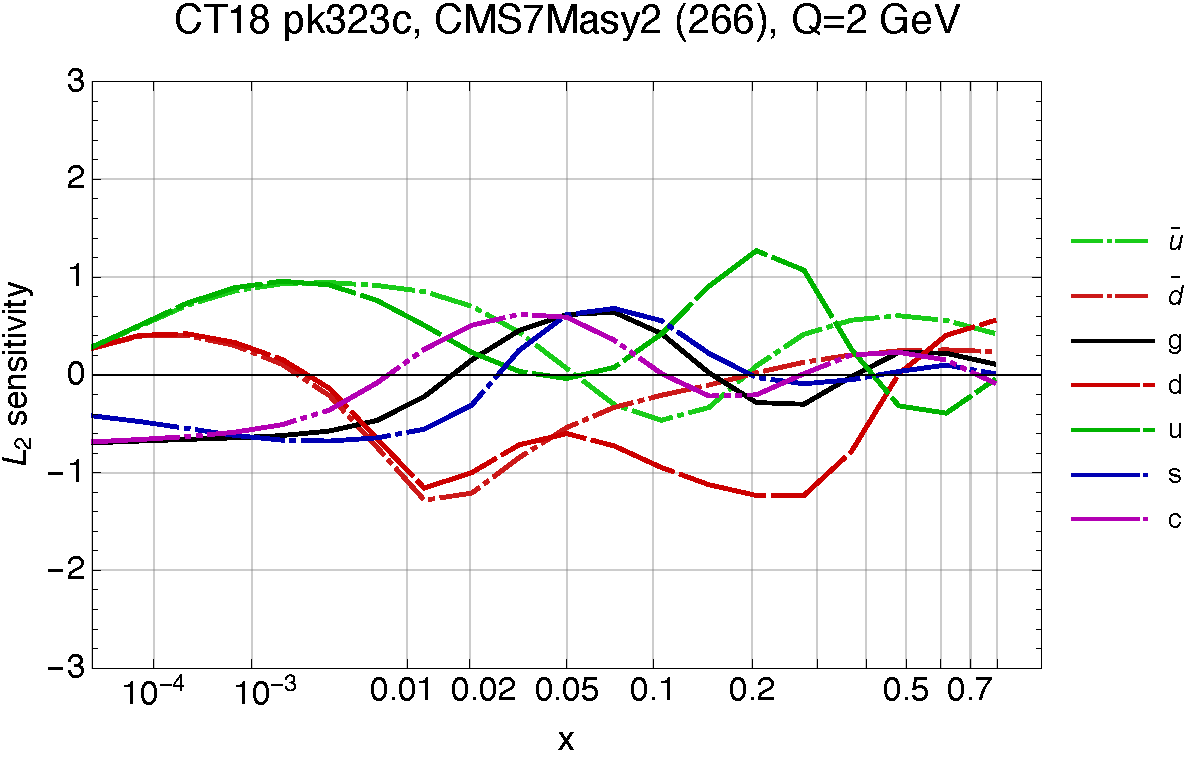
\includegraphics[width=\textwidth,height=0.44\textheight,keepaspectratio]{266_ct18nn_L2_q2_Sf_1.pdf}
\caption{\protect{266\_ct18nn\_L2\_q2\_Sf\_1.pdf}}
\end{figure}
\begin{figure}
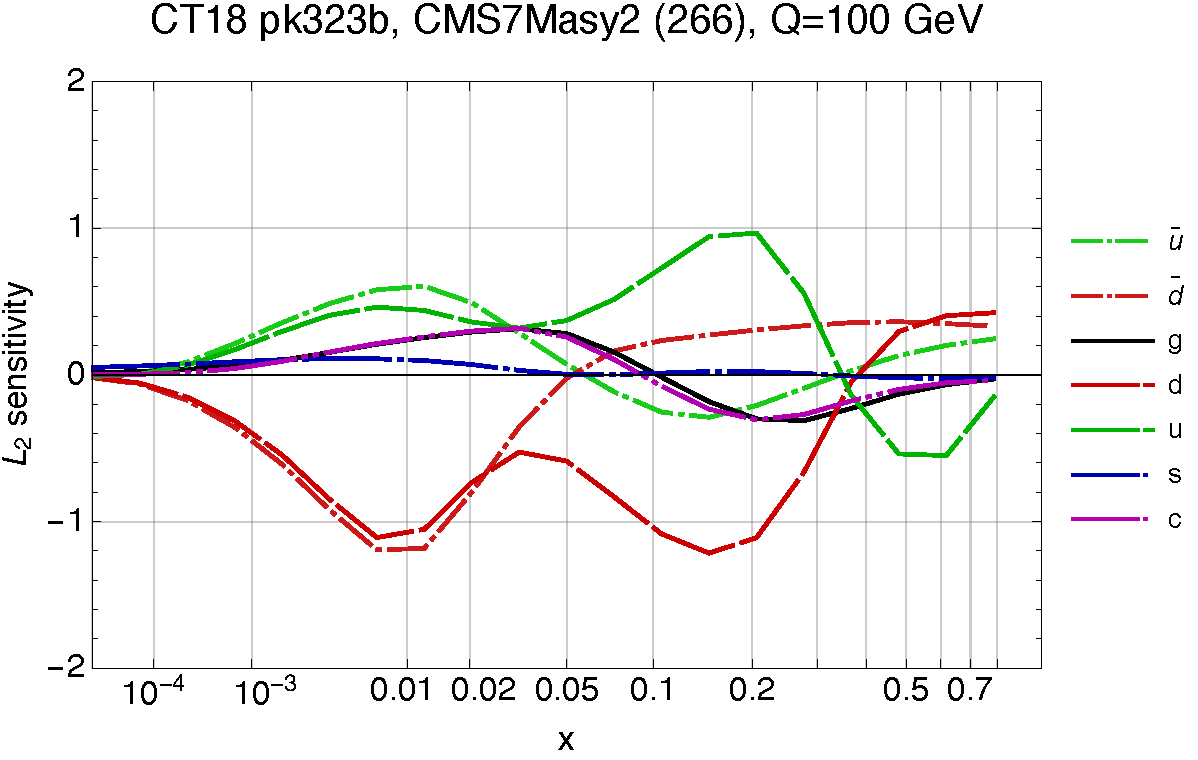
\includegraphics[width=\textwidth,height=0.44\textheight,keepaspectratio]{266_ct18nn_L2_q100_Sf_1.pdf}
\caption{\protect{266\_ct18nn\_L2\_q100\_Sf\_1.pdf}}
\end{figure}
\clearpage
\begin{figure}
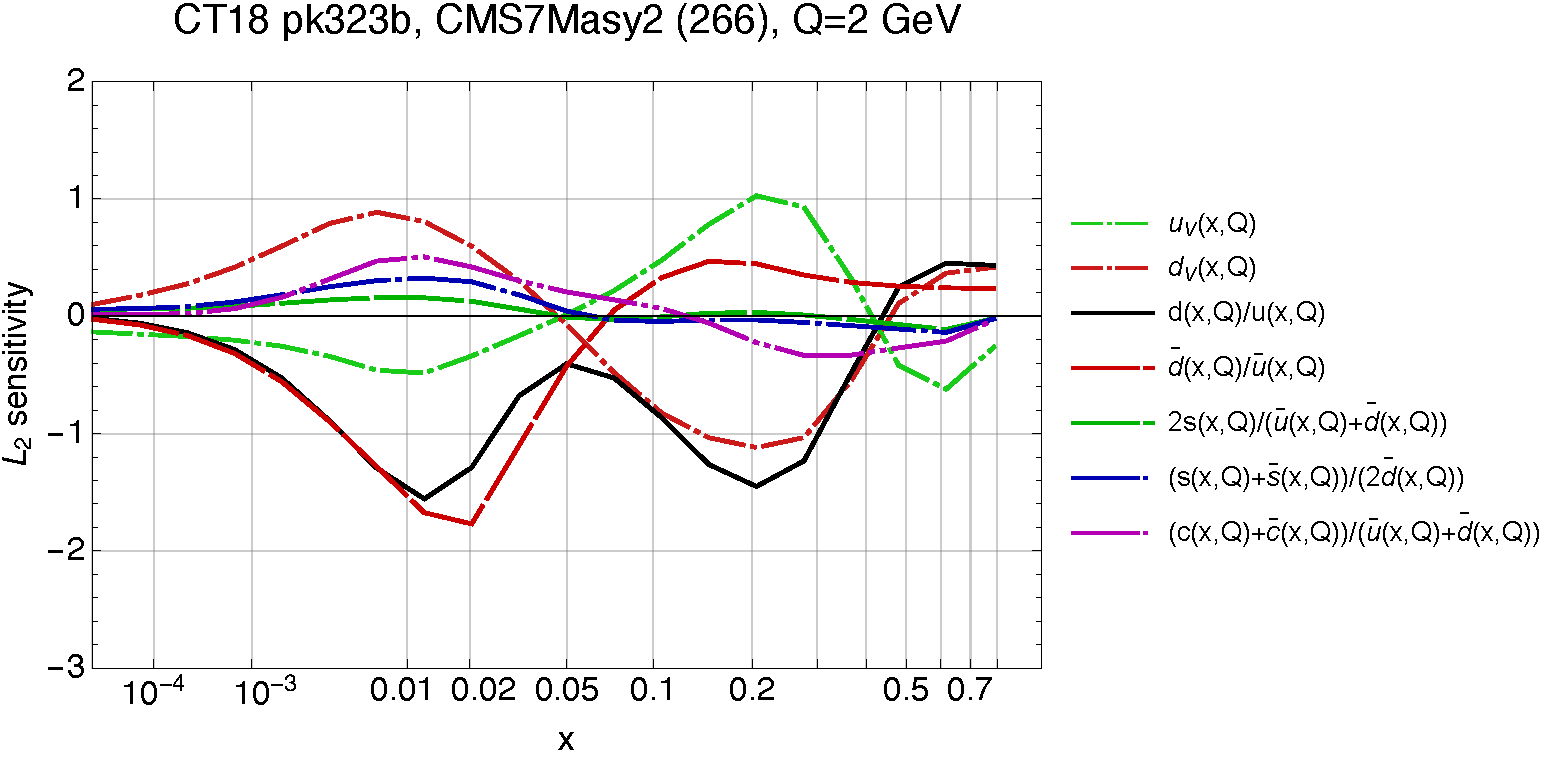
\includegraphics[width=\textwidth,height=0.44\textheight,keepaspectratio]{266_ct18nn_q2_Sf_2.pdf}
\caption{\protect{266\_ct18nn\_q2\_Sf\_2.pdf}}
\end{figure}
\begin{figure}
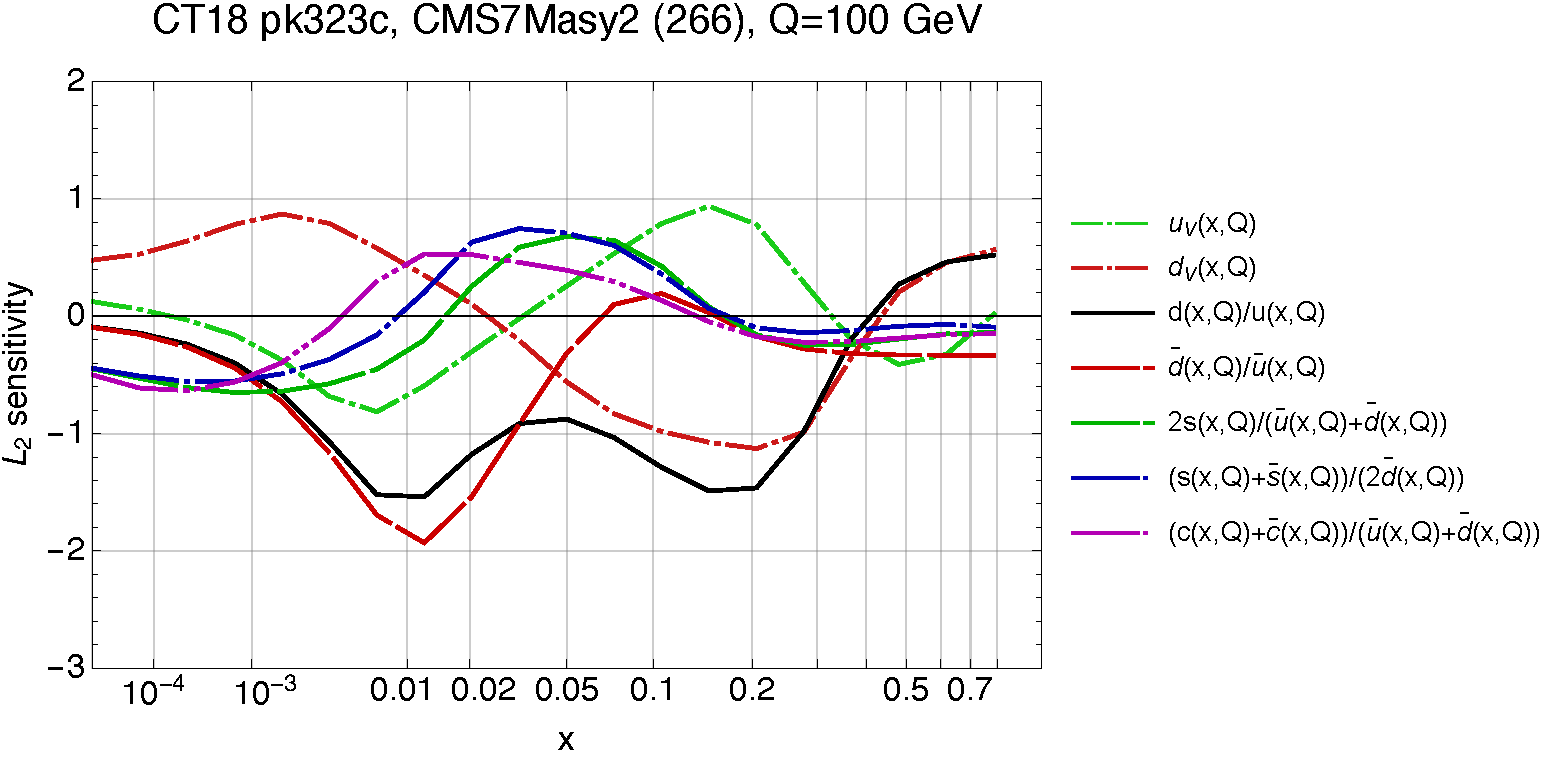
\includegraphics[width=\textwidth,height=0.44\textheight,keepaspectratio]{266_ct18nn_q100_Sf_2.pdf}
\caption{\protect{266\_ct18nn\_q100\_Sf\_2.pdf}}
\end{figure}
\clearpage
\end{document}
